\medskip

\begin{enumerate}
\item \begin{enumerate}
		\item La fonction exponentielle est continue sur $\R$ donc :\quad $\lim\limits_{x \to 1} \e^{x} = \e^1 = \e >0$.

		Par limite de la somme, on a :\quad $\lim\limits_{x \to 1} x - 1 = 0$, et comme on travaille sur $]-\infty~;~ 1[ $, on a $x - 1 < 0$. (on peut noter $\lim\limits_{x \to 1} x - 1 = 0^-$ ).

		Par limite du quotient, on a :\quad $\lim\limits_{x \to 1} f(x) = -\infty$.

		\item On en déduit que la courbe $ \mathcal{C} $ admet une asymptote verticale, d'équation $x = 1$.

	\end{enumerate}
	\item On a : \quad $\lim\limits_{x \to -\infty} \e^x = 0$;

	Par limite de la somme, on a :\quad $\lim\limits_{x \to -\infty} x - 1 =-\infty$,

	Par limite du quotient, on en déduit :\quad $\lim\limits_{x \to -\infty} f(x) = 0$.

	On en déduit que $ \mathcal{C} $ admet également une asymptote, d'équation $y = 0$, au voisinage de $ -\infty $.

\item \begin{enumerate}
		\item $f$ est dérivable sur $ ]-\infty ~;~ 1[ $, en tant que quotient de fonctions définies et dérivables sur cet intervalle, avec la fonction au dénominatuer ne s'annulant pas sur l'intervalle.

		$\begin{aligned}[t] \forall x \in ]-\infty~;~1[ ,\quad f'(x) & = \dfrac{\e^x \times (x - 1) - \e^x \times 1}{(x-1)^2 }\\
		&= \dfrac{\e^x \times (x - 1 - 1)}{(x-1)^2}\\
		&= \dfrac{(x - 2)\e^x}{(x - 1)^2}\\ \end{aligned}$

		\item La fonction exponentielle est à valeurs strictement positives sur $\R$, et pour tout $x$ dans $ ]-\infty ~;~ 1[ $, $(x - 1)^2$ est strictement positif, donc le signe de $f'(x)$ est le même que le signe de $(x - 2)$.

$x - 2 \geqslant 0 \iff x \geqslant 2$, donc sur $ ]-\infty ~;~ 1[ $, $(x-2)$ est  strictement négatif, donc $f'(x)$ également.

Finalement, on peut donc en déduire que $f$ est strictement décroissante sur $]-\infty ~;~ 1[$, et donc, on a le tableau de variations suivant (avec les limites justifiées aux questions \textbf{1. a.} et \textbf{2.}):

\begin{center}
			\begin{tikzpicture}
			\tkzTabInit[lgt=3, espcl=4]{$x$/0.8,signe de $f'(x)$/0.8,variations de $f$/1.5}{$ -\infty $ , 1}
			\tkzTabLine{t,-,d}
			\tkzTabVar{+/0,-D/$-\infty$}
			\end{tikzpicture}
\end{center}
	\end{enumerate}

\item \begin{enumerate}
		\item Pour étudier la convexité de la fonction $f$ sur l'intervalle $]-\infty~;~1[$, on va étudier le signe de $f''(x)$.

		Comme, pour tout $x$ dans $ ]-\infty ~;~1[ $, on a $(x - 1) < 0$ et donc $(x - 1)^3 < 0$ et $\e^{x} > 0$, on en déduit que le signe de $f''(x)$ est l'opposé du signe du trinôme : $x^2 - 4x + 5$.

Or, ce trinôme a un discriminant $\Delta = (-4)^2 - 4 \times 1 \times 5 = -4 $ qui est strictement négatif, donc n'admet pas de racine, et donne des images strictement positives (car le coefficient dominant est positif) pour tout réel $x$.

\emph{Rem.} On peut écrire :

$x^2 - 4x + 5 = (x - 2)^2 - 4 + 5 = (x - 2)^2 + 1 \geqslant 1 > 0$ : le trinôme est positif quel que soit $x \in \R$.

Finalement, la dérivée seconde $f''$ est à valeurs strictement négatives sur $\left]-\infty ~;~ 1\right[$, on en déduit que la fonction $f$ est concave sur $]-\infty ~;~ 1[$.

		\item Pour déterminer l'équation de $T$, il nous faut connaître $f'(0)$ et $f(0)$ :

\begin{itemize}[left=5mm]
\item $f'(0) = \dfrac{(0 - 2)\e^{0}}{(0 - 1)^2} = \dfrac{-2}{1} = -2$;
\item $f(0) = \dfrac{\e^0}{0 - 1} = \dfrac{1}{-1} = -1$.
\end{itemize}

La formule classique donne une équation pour $T$ :

$y = f'(0)(x - 0) + f(0) \iff y = - 2x - 1$

L'équation réduite de $T$ est donc : $y = - 2x - 1$.

		\item Puisque $f$ est concave sur l'intervalle $]-\infty~;~1[$, la courbe $\mathcal{C}$ est donc située sous ses tangentes, notamment sous la tangente $T$, sur cet intervalle.

Pour tout réel $x$ dans cet intervalle, l'ordonnée d'un point sur la courbe $\mathcal{C}$ (c'est-à-dire $f(x)$) est donc inférieure ou égale à l'ordonnée du point ayant la même abscisse sur la tangente $T$ (or, sur la tangente $T$, l'ordonnée du point d'abscisse $x$ est $- 2x -1$, d'après la question précédente).

On en déduit donc : \quad $\begin{aligned}[t] x \in ]-\infty~;~1[ &\implies f(x) \leqslant -2x -1\\
		&\implies \dfrac{\e^x}{x - 1}\leqslant - 2x - 1\\
		&\implies \e^x \geqslant (x -1)(-2x-1)\\
		& \qquad \quad \text{car sur }]-\infty ~;~ 1[,\quad x - 1 <0\\
		&\implies \e^x \geqslant (-2x - 1)(x - 1)
		\end{aligned}$

On arrive donc à l'inégalité demandée.
	\end{enumerate}
\item
	\begin{enumerate}
		\item La fonction $f$ est :
		\begin{itemize}[left = 5mm]
			\item continue sur $]-\infty~;~1[$ (car dérivable sur cet intervalle);
			\item strictement décroissante sur $]-\infty~;~1[$ (d'après la question \textbf{3. b.});
			\item telle que $-2$ est une valeur intermédiaire entre $\lim\limits_{-\infty} f = 0$ et $\lim\limits_{1} f = -\infty$;
		\end{itemize}
		D'après le corollaire du théorème des valeurs intermédiaires appliqué aux fonctions strictement monotones, l'équation $f(x) = -2$ admet une unique solution $\alpha$ sur l'intervalle $]-\infty~;~1[$.

		\item Comme on a repéré à la question \textbf{4. b.} que $f(0) = -1$, on sait que la solution sera à chercher dans l'intervalle $]0 ~;~ 1[$.

À l'aide de la calculatrice, par balayage, on a :
\begin{itemize}[left=5mm]
\item $f(0,31) \approx -1,98 > -2$;
\item $f(0,32) \approx-2,03 < -2$;
\end{itemize}

Un encadrement de $\alpha$ d'amplitude $10^{-2}$ est $0,31 < \alpha < 0,32[$.
	\end{enumerate}
\end{enumerate}

\medskip
